% !TEX root =  master.tex
\chapter{Projektmanagement}
	
	\section{Projektdefinition}
	Das Ziel des Projektes \ac{ICS} ist die Entwicklung eines Prototypen für die Online-Reservierung von Kino-Tickets. Das Projekt wird mit der vorliegenden Seminararbeit dokumentiert. Mit der Abschlusspräsentation am 12.02.2019 ist das Projekt zu Ende.
	
	\section{Projektbeteiligte}
	An dem Projekt \ac{ICS} arbeiten acht Personen des Kurses WWI 17 SE B der Dualen Hochschule Baden-Württemberg in Mannheim. Im Rahmen der Lehrveranstaltung \enquote{Fallstudie} des Moduls \enquote{Umsetzung der Methoden der Wirtschaftsinformatik} legen folgende Studenten ihre Prüfungsleistung ab:
	\begin{singlespacing}
	\begin{itemize}
		\item Dutzi Jonas, Matrikelnummer: 6681598
		\item Keller Sandra, Matrikelnummer: 6046520 
		\item Köhler Dennis, Matrikelnummer: 8900967 
		\item Sandig Martin, Matrikelnummer: 8857640 
		\item Waage Felix, Matrikelnummer: 3459154 
		\item Werner Yvonne, Matrikelnummer: 8519757 
		\item Westphal Fabio, Matrikelnummer: 6198411  
		\item Zahn Milena, Matrikelnummer: 7488221 
	\end{itemize}
	\end{singlespacing}

	\section{Feasibility Study}
	Bevor das Projekt \ac{ICS} gestartet ist, wurde zuerst eine Feasibility Study/ Machbarkeitsstudie durchgeführt. Es wurde geprüft, ob alle erforderlichen Voraussetzungen für das Projekt vorhanden sind. Die in dem ersten Studienjahr vermittelten programmiertechnischen sowie methodischen Grundlagen werden angewandt. Durch die Lehrveranstaltung \textit{Systemanalyse und -entwurf} des zweiten Semesters wurden alle notwendigen Kompetenzen zur objektorientierten Analyse und Entwurf erworben. Durch das Modul \textit{Programmierung und Programmiertechniken} des ersten und zweiten Semesters kann man Erfahrung in der Programmiersprache Java voraussetzen. Vor dem Projektstart wurden die Rahmenbedingungen, unter denen das Projekt laufen soll, von dem Dozenten gegeben. Des Weiteren wurde innerhalb der Gruppe besprochen, inwiefern das Projekt in der gegeben Zeit umgesetzt werden kann. Der Prozess, dass unterschiedliche Personen sinnvoll zusammenwirken und vielfältige Fähigkeiten  ausgeglichen werden, stellt eine Herausforderung dar.
	
	Unter Berücksichtigung der Bedingungen dieses Projekts ist vor allem der enge Zeitrahmen auffällig. Das Projektmanagement ist somit neben der Implementierung des Kino-Reservierungstools eine sehr wichtige Aufgabe. Parallel zu diesem Projekt müssen Prüfungsleistungen sowie Vorlesungen von anderen Modulen des dritten Semesters absolviert und demnach mit berücksichtigt werden. Um diese einzuplanen und ein erfolgreiches Projekt abzuschließen, ist eine Projektplanung essentiell. Aus diesen Gründen wurde das Projektmanagement von Anfang an von allen Teammitgliedern durchgeführt und beachtet.
	
	\section{Projektplanung} \label{projektplan}
	\subsection{Projektzeitplan}
	In Abbildung \vref{fig:projektablauf} wird der vor Projektablauf zu Beginn des Projektes dargestellt. Das Projekt beginnt am 26.11.2018 und endet am 12.02.2019. Innerhalb dieser zwölf Wochen sind drei Iterationen vorgesehen. Im Rahmen einer kurzen Präsentation in KW51 2018 und KW4 2019 werden die in der jeweiligen Iteration erarbeiteten Ergebnisse dem Dozenten Kurs sowie dem vorgestellt. Ziel dieser Präsentationen ist es, den aktuellen Projektstatus vorzustellen sowie Feedback einzuholen. Außerdem dienen diese Präsenzen dazu, Fragen zu stellen oder sonstige Hindernisse zu klären. 
	\begin{figure}[H]
		\centering 
		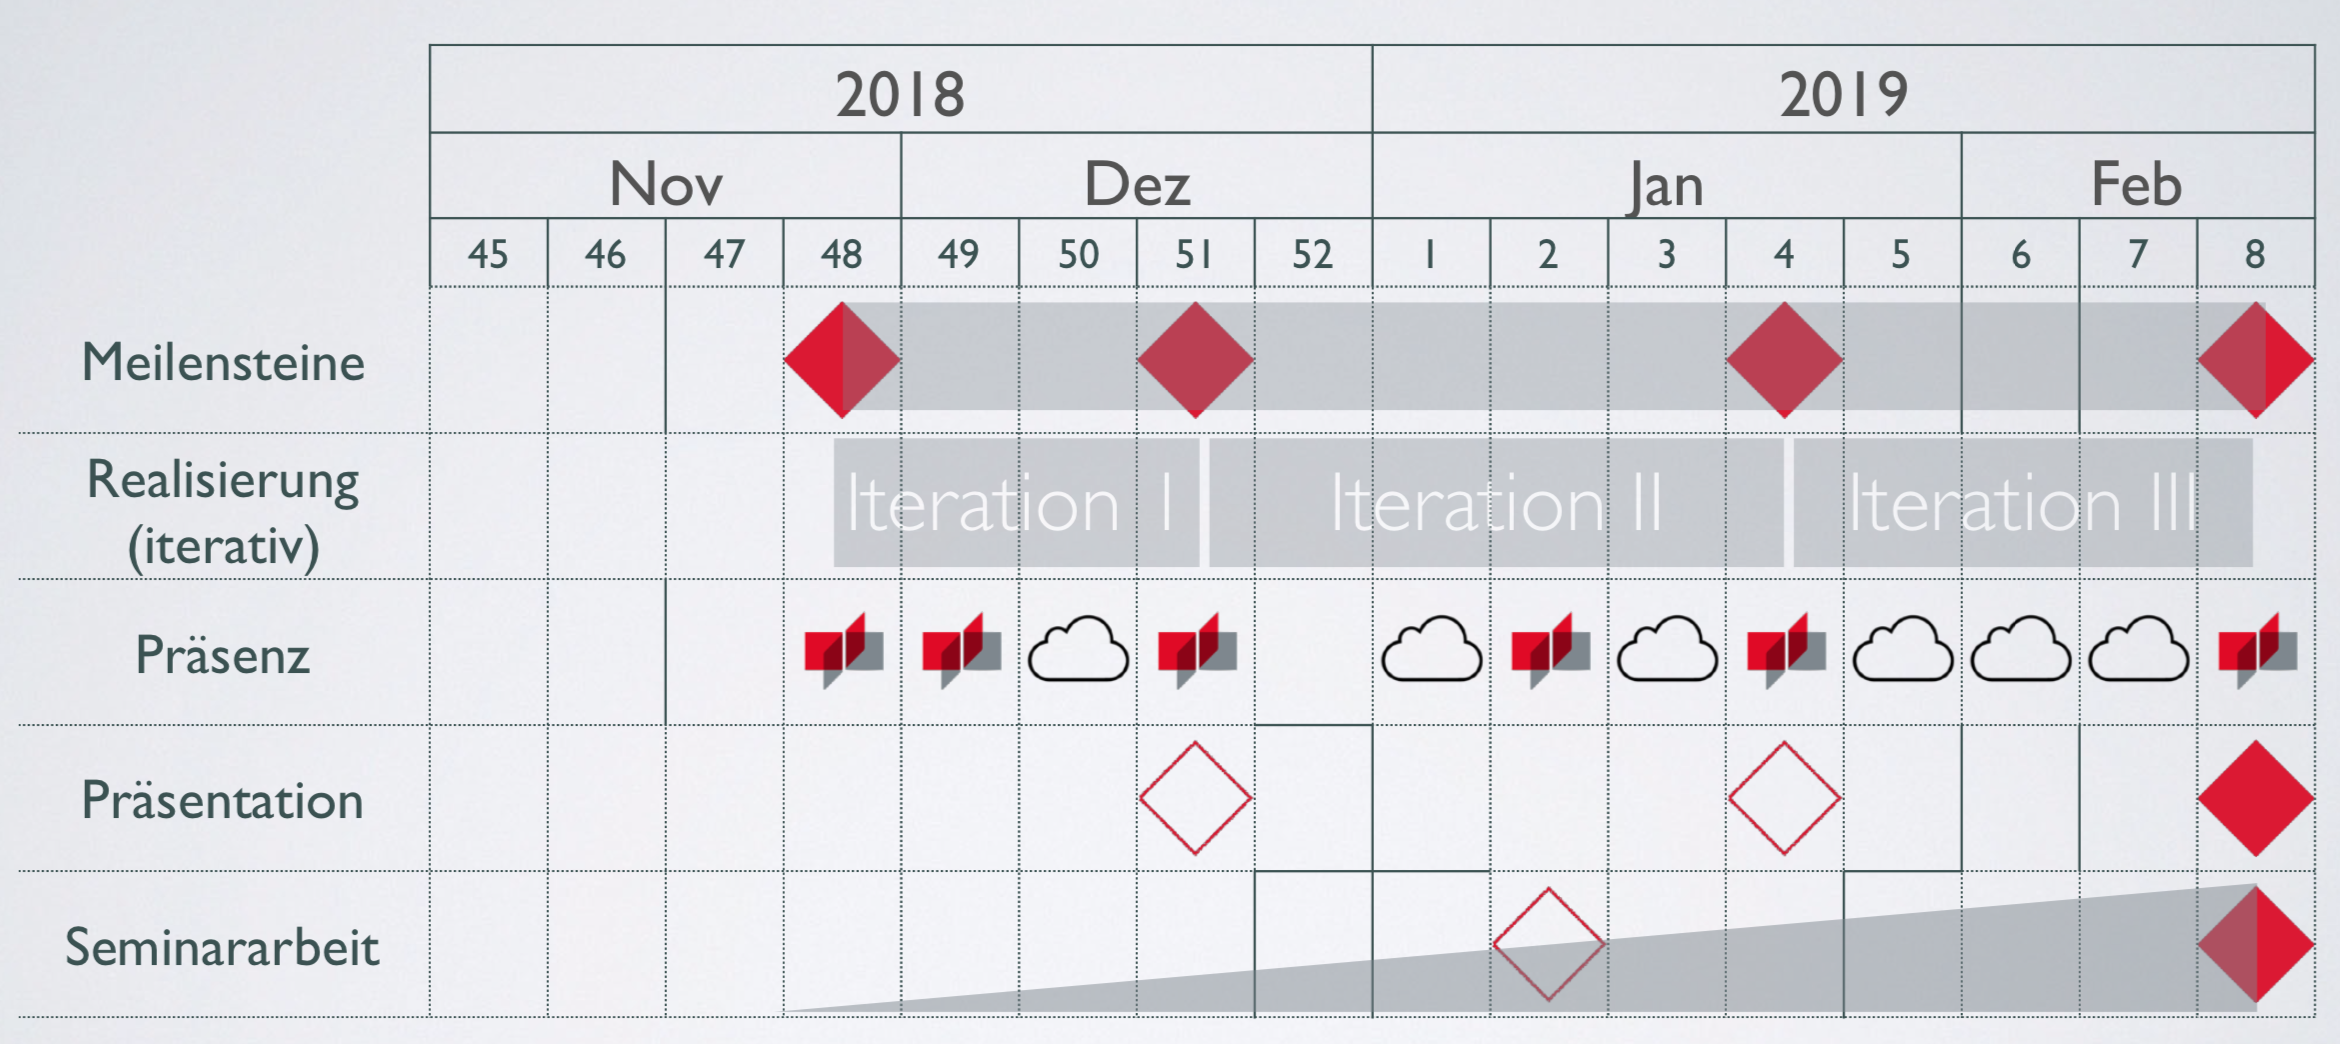
\includegraphics[scale=0.3]{img/geplanterProjektablauf.png}
		\captionsetup{format=hang}
		\caption[Geplanter Projektablauf ]{\label{fig:projektablauf} Geplanter Projektablauf \\ Quelle: Skript, Gregor Tielsch }
	\end{figure}
	
	\subsection{Projektplanung mit Gantt Diagramm}
	Der Projektplan ist das zentrale Dokument des Projektmanagements, da er den Projektfortschritt unterstützt und alle Aufgaben enthält, die innerhalb dieses Projektes zu erledigen sind. Das Projektmanagement wurde für das gesamte Projekt durchgeführt. Die Hauptaktivitäten des Projekts sind in der Abbildung \vref{fig:projektplan} dargestellt. Das Gantt Diagramm wurde stets während der Durchführung des Projektes gepflegt, um den aktuellen Projektfortschritt zu dokumentieren und das fristgerechte Erreichen des Projektzieles sicherzustellen. In regelmäßigen Projektsitzungen wurde der Projektfortschritt über das Gantt Diagramm sowie die Meilensteile überwacht und dokumentiert. So ist der Projektstatus jederzeit transparent und für alle Teammitgliedern ersichtlich. Dadurch kann gegebenenfalls eingegriffen werden, wenn Meilensteine nicht erreicht werden und das Projekt in Gefahr läuft in Verzug zu geraten.  
	Um den Projektplan jedem Teammitglied jederzeit zur Verfügung zu stellen, wurde entschieden das Gantt Diagramm mit der online Planungssoftware \enquote{Tom's Planner}\footnote{https://www.tomsplanner.de} zu erstellen. Zu Beginn des Projektes wurden die Meilensteine in Orientierung an den Projektablaufplan Abbildung \vref{fig:projektablauf} angelegt. 
	\begin{figure}[H]
		\centering 
		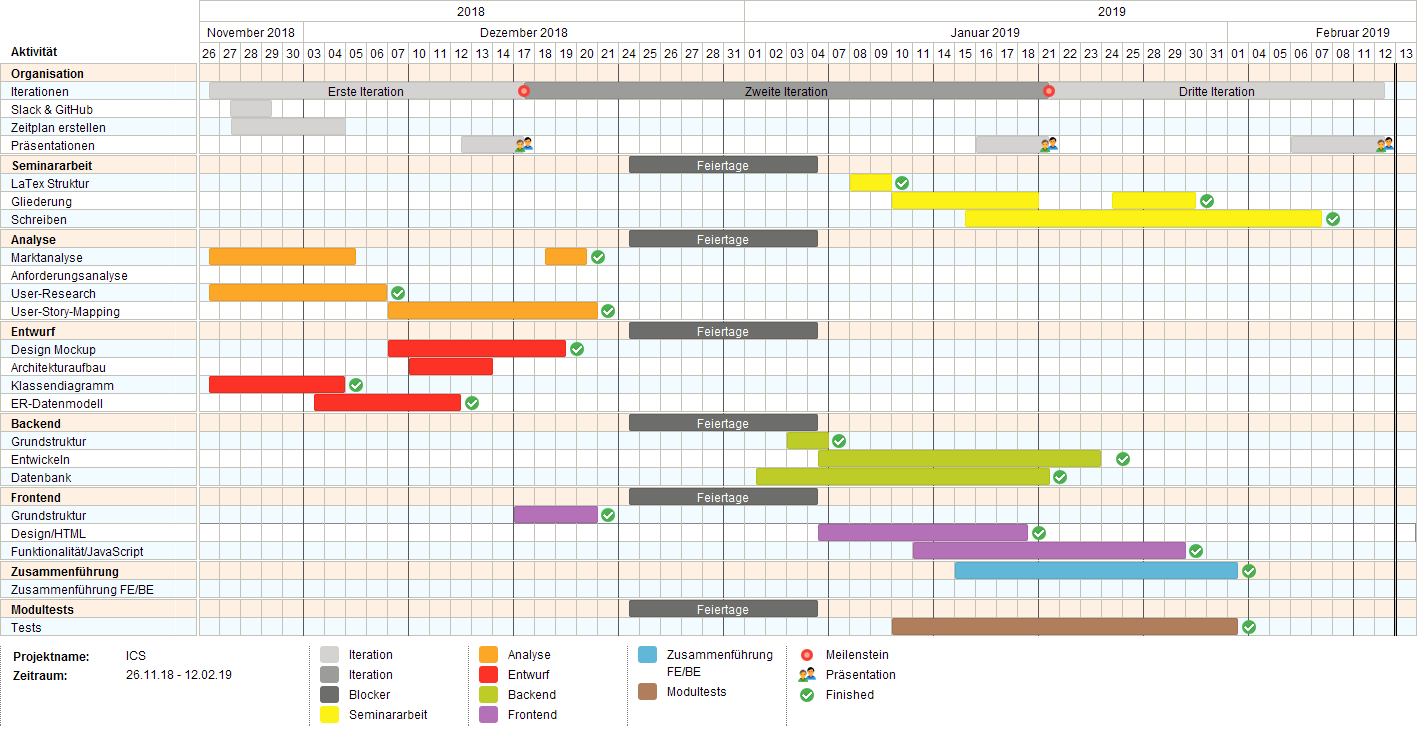
\includegraphics[scale=0.3]{img/projektplan.png}
		\captionsetup{format=hang}
		\caption[Projektplan]{\label{fig:projektplan} Projektplan ICS, Gantt-Diagramm[DRAFT - unvollständig/zu klein] \\ Quelle: Tom's Planner}
	\end{figure}
	Die aktuell bearbeiteten Aufgaben wurden kontinuierlich in das Gantt Diagramm eingetragen, damit eine Übersicht entsteht, wann und wie lange an der jeweiligen Aufgabe gearbeitet wurde. Zunächst wurden einige organisatorische Aufgaben erledigt sowie ein Organisations-Tool eingerichtet. Die Organisation des Teams wird in Kapitel \vref{teamorga} genauer erläutert. Die Analyse (Kapitel \vref{analyse}) sowie der Entwurf (Kapitel \vref{entwurf}) wurden in der ersten Interation erarbeitet. Wobei die Marktanalyse in der zweiten Iteration erneut durchgeführt wurde, da zu diesem späteren Zeitpunkt neue Probleme aufgetreten sind. Nachdem das Grundkonzept der Anwendung durch ein Mockup und dem Design der Softwarearchitektur festgelegt wurde, wurde das Backend und das Frontend entwickelt. Dies wird im Kapitel \vref{umsetzung} detaillierter erklärt. In der zweiten und letzen Iteration wurde parallel zu der Entwicklung die Seminararbeit geschrieben. Gegen Ende der dritten Iteration wurde schließlich der Fokus auf die Präsentation sowie die Fertigstellung der Seminararbeit gelegt. Das Projekt endete am 12.02.2019 mit dem letzten Meilenstein \enquote{Abschlusspräsentation}.
	
	
	\section{Teamorganisation} \label{teamorga}
	Eine wichtige Kompetenz innerhalb dieses Projektes ist es, sich selbst sowie das Team zu organisieren, um in dem begrenzten Zeitraum mit den gegebenen Resssourcen das Projektziel zu realisieren. Die Effizienz des Informationsaustausches und der Kommunikation innerhalb des Teams bestimmt wesentlich dessen Erfolg mit. Aus diesem Grund wurde das Kommunikationstool \enquote{Slack}\footnote{https://slack.com/} gewählt. Die Projektbeteiligten sind alle mit dem Programm, unter anderem durch die Lernveranstaltung \textit{Systemanalyse und -entwurf} und durch die Praxisphasen, vertraut, wodurch eine Einarbeitungszeit eingespart werden kann. Für das Projekt wurde ein eigener Workspace angelegt. Kurze Teamabsprachen sowie Fragestellungen innerhalb des Teams, konnten damit schnell online geklärt werden. Ein weiterer Vorteil von Slack ist die Transparenz, die durch die verschiedenen, offenen Channels gegeben wird. Durch \enquote{Slack} wurde ein stetiger, unkomplizierter Dialog unter den Teammitgliedern ermöglicht.
	